\documentclass[12pt]{article}
\usepackage{graphicx}
\graphicspath{{./figs/}}{}
\usepackage{amsmath,amssymb,amsfonts,amsthm}
\newcommand{\myvec}[1]{\ensuremath{\begin{pmatrix}#1\end{pmatrix}}}
\usepackage{listings}
\usepackage{watermark}
\usepackage{titlesec}
\let\vec\mathbf
\lstset{
frame=single, 
breaklines=true,
columns=fullflexible
}
\thiswatermark{\centering \put(0,-105.0){
\includegraphics[scale=0.15]{logo2.png}} }
\title{\mytitle}
\title{
Assignment - Vector
}
\author{Surajit Sarkar}
\begin{document}
\maketitle
\tableofcontents
\bigskip
\section{\textbf{Problem}}
Find the distance between the point(0,0) and (36,15).Can you now find the distance between the two towns A and B discussed in Section 7.2
\section{\textbf{Solution}}
The distance betwen the points A and B is given
\begin{equation}
    \Vec A=\myvec{0 & 0}
\end{equation}
\begin{equation}
    \Vec B=\myvec{36 & 15}
\end{equation}

\begin{equation}
   \|\vec {A-B}\|
\end{equation}
where
\begin{equation}
    \vec {A-B}=\myvec{-36\\-15}
\end{equation}
\begin{equation}
    \vec d=\sqrt{\myvec{\vec {A-B}}^T\myvec{\vec {A-B}}}
\end{equation}
\begin{equation}
    \Vec d =\sqrt{\myvec{-36\\-15}{\myvec{-36-15}}}
\end{equation}
\begin{equation}
    \vec d=\sqrt{1296+225}
\end{equation}
\begin{equation}
    \vec d=\sqrt{1521}
\end{equation}
\begin{equation}
    \vec d=39
\end{equation}
\section{\textbf{Figure}}
\begin{figure}[h]
    \centering
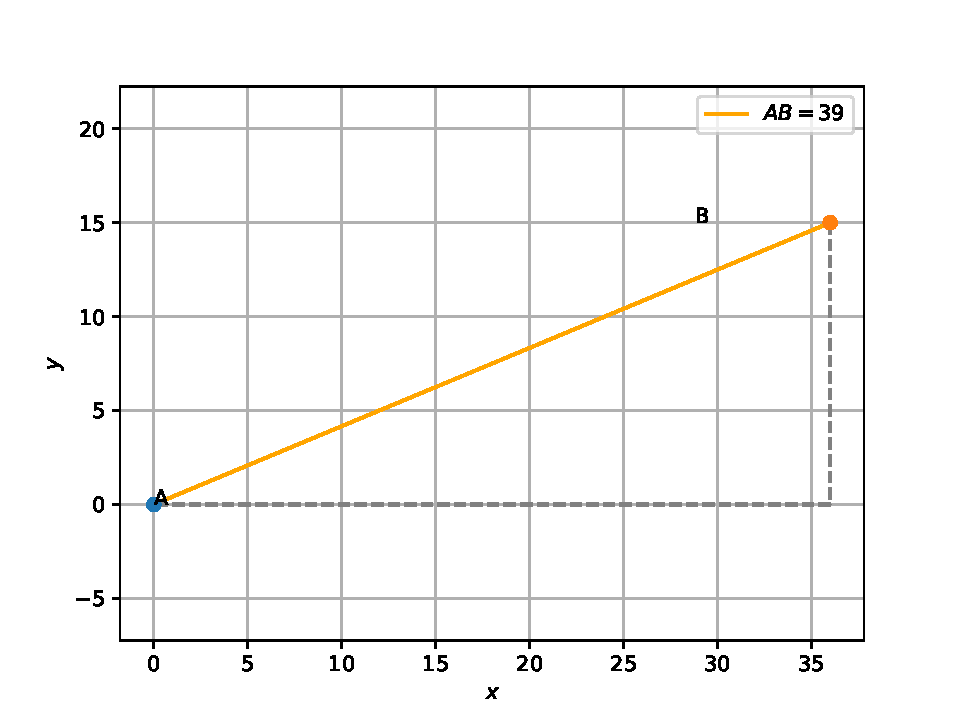
\includegraphics[width=\columnwidth]{vec.pdf}
    \label{fig:my_label}
\end{figure}
\section{\textbf{Code Link}}
\begin{lstlisting}
https://github.com/sssurajit/fwc/blob/main/vector/codes/vector.py
\end{lstlisting}
Execute the code by using the command\\
\textbf{python3 vector.py}
\end{document}
